\chapter{The instance classes}

%final
If the author of this work could suggest one single thing to be improved in the future works about UKP, it would be the selection of the instances.

%working
The UKP is a variation of the classic knapsack problem, with the difference that an unbounded number of each item is available.

The study of the UKP has fallen in one of the pitfalls described by David Johnson in his guide to 

%pending
the ukp seems like a problem that should have many applications, but <CITE PYAsUKP 'are hard to find'>
the most classical real-world use of the problem is the unidimensional cutting stock problem 
	explain the problem
	explain how branch and price can be used to solve the problem
	cite gilmore and gomory (and brevily point that UKP5 and ordered step-off are very similar, more will be said in the algorithms section)
point error in the article, the pure UKP can only be used to solve the root node of the cutting stock exact continuous relaxation
the best solver don't use UKP anymore at all, but one of the good solvers use it, and repoted that in some cases, about 70\% of the processing is done at the root node

the use of artificial instances was already strongly crticized in the past
the reasons for their use is the possibility of generating many instances, of many sizes (what allows for examinating the growth of the time with the growth of the instance)
	This is specially interesting for UKP because it's one of the easiest NP-Hard problems, so big instances or hard instances have to be used to get high execution times, small execution times are too much affected by variance
	yet, artificial instances should not be used at all, if there's no guarantee that the growth/time/results will translate for real world instances (i.e. artificial instances should follow )

	The paper are the hard knapsack problems shows that even for 0-1 knapsack instances (that are by default harder than UKP instances), the instances used were easy to solve


The major problem with an experimental analysis of the UKP solving methods over artificial instances is that the different solving approaches are affected by the items distributions (i.e. some methods are the best for some for some distributions and the worst for others). Consequently, the results aren't useful for someone that wants to tackle real world UKP instances, unless some artificial instance distribution ends up modelling the 

TODO: The use of testbeds is overrated?

We have already pointed (TODO: refer to timeline) that the choices of item distributions on the generation of artificial instances in the previous literature has defined what was considered the best algorithm. I have written two sections of this chapter to further illustrate this point. Those are sections are (TODO: refer to) uncorrelated instances, and the second is the BREQD instances. The former points (TODO: list things pointed in uncorrelated instances); the latter presents a new instance distribution, that's easy to solve by B\&B methods and hard to solve by DP methods (some experimental results over this classes of instances will be presented at TODO: refer).

\section{Uncorrelated Random Coeficients Instances}

In this work, the expression `uncorrelated instances' will be used to refer to a family of UKP instances where the weight and the profit of an item have no correlation. The most common way for generating those uncorrelated instances is generating a value between \(w_{min}\) and \(w_{max}\) for the weight, and a value between \(p_{min}\) and \(p_{max}\) for the profit, for each of the \(n\) items of the instance using a (pseudo-)random number generator with an uniform distribution. %Uncorrelated instances can be generated using a (pseudo-)random number generator to generate \(n\) numbers between \(w_{min}\) and \(w_{max}\), and another \(n\) numbers between \(p_{min}\) and \(p_{max}\). Sorting both arrays will give (TODO: refer to realistic instances), that is another instance type. Uncorrelated instances 

PUTS IMAGE
\begin{figure}
    \caption{An uncorrelated instance generated with \(n = 100\), \(w_{min} = 1\), \(w_{min} = 1000\), \(p_{min} = 1\), and \(p_{max} = 1000\).}
    \begin{center}
    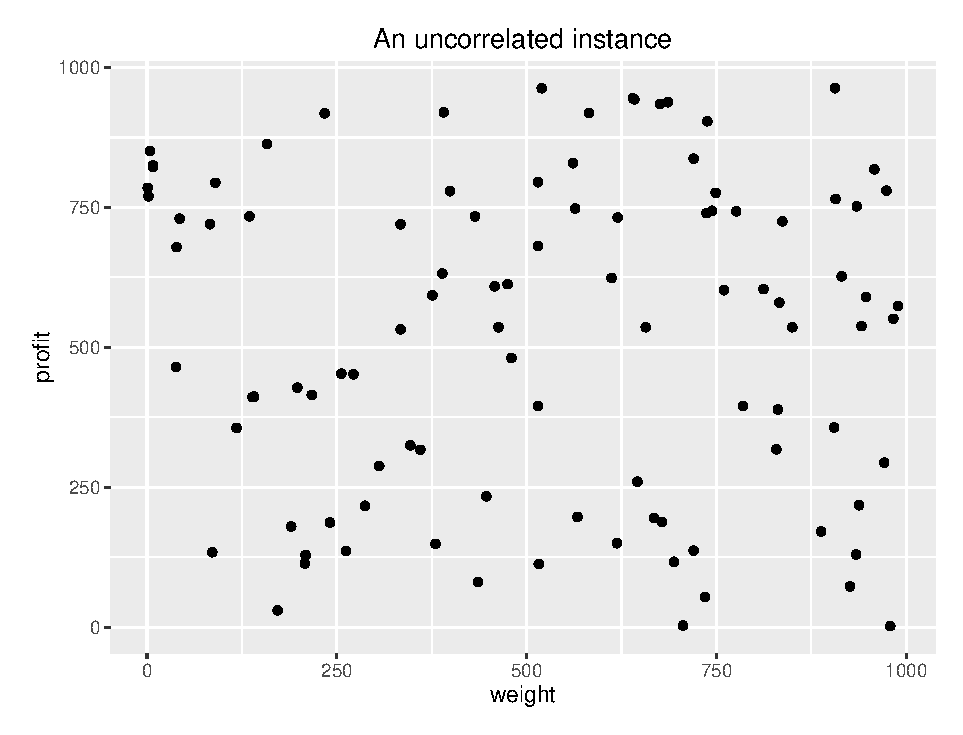
\includegraphics[scale=1]{uncorrelated.eps}
    \end{center}
    \legend{Source: the author.}
    \label{fig:uncorrelated_example}
\end{figure}

Expose why they are uninteresting: we do not know if they model any real world instance; it's a simple matter of running a good polynomial simple/multiple dominance algorithm first, or using MTU2 that was developed for this purpose. Increasing values of \(n\) increase the time taken by MTU2 or dominance removal in a polynomial fashion. The NP-hard part of the problem, that is finding an optimal solution between non-dominated items don't grow with \(n\). %(sorting or the \(O(n^2)\) dominance algorithms).

\section{Bottom Right Ellipse Quadrant Instances}

The Bottom Right Ellipse Quadrant Instances (`BREQ instances', for short) is a new item distribution proposed by the author in this work. This instance distribution was created to illustrate that different item distributions favor different solution approaches and, therefore, the choice of instances (or specifically, their item distribution) defines what is considered the `best algorithm'. Distributions that are easy to solve by the DP approach and hard to solve by the B\&B approach are common (i.e. many with this characteristic have been proposed in the literature). This distribution has the opposite trait, is hard to solve by DP and easy to solve by B\&B. It's important to point that this is an artificially generated distribution that don't model any real world instances (that the author have knowledge). The author discourages the use and study of such instances and created this distribution only as a tool to prove a point; research should focus on real-world instances and/or artificially generated instances that clearly model real world instances.

The gist of this distribution is that, when plotted on a graph, the instance items show the form of a quarter of ellipse (specifically the bottom right quadrant). A natural consequence of that distribution shape is that the item profit and efficiency grows quadratically with the item weight. This leads to the inexistance of simple, multiple and collective dominance\footnote{In truth, if the profit is integer, the smallest items can display some of those three dominances because the profit has to be rounded, but this is of little relevance and can be safely ignored for most purposes}. In other words, for any multiset of items \(s\) and any single item \(i\) (with respective weigths \(w_s\) and \(w_t\), and respective profits \(p_t\) and \(p_i\)), if \(w_s \leq w_i\) then \(p_s < p_i\).

\section{Uncorrelated Random Coeficients Instances}

\section{Chung}
% TEX COPIED FROM SEA 2016 article, CHANGE AND AMPLIFY

\section{PYAsUKP instances}

This section will discuss the instance sets used in~\cite{pya}.
The distributions used by the instances weren't novel, but a 
Those instance sets were artificially generated with the purpose of being ``hard to solve'', what means a different thing for each one of them.


The same tool was used to generate the datasets (PYAsUKP), and the same parameters were used, otherwise noted the contrary. 
In Subsection 5.1.1 \emph{Known ``hard'' instances} of~\cite{pya} some sets of easy instances are used to allow comparison with MTU2. 
However, the authors reported integer overflow problems with MTU2 on harder instances. 
With exception of the subset-sum dataset, all datasets have a similar harder set (Subsection 5.2.1 \emph{New hard UKP instances}~\cite{pya}).
Thus, we considered in the runs only the harder ones. 
Each instance has a random capacity value within intervals shown in Table~\ref{tab:times}. 
The PYAsUKP parameters \mbox{\emph{-wmin \(w_{min}\) -cap c -n \textbf{n}}} were used in all instances generation. 
%When we found a discrepancy between the formula presented in \cite{pya} and the PYAsUKP code, or generated instances, we opted for changing the formula based on the observed behavior. 
%As our knowledge of OCaml is limited, we cannot guarantee that the formula presented here is a perfect match for the code; but, based by the generated instances, we believe it to be correct to a good extent.
We found some small discrepancies between the formulas presented in~\cite{pya} and the ones used in PYAsUKP code.
We opted for using the ones from  PYAsUKP code, and they are presented below.

\subsubsection{Subset-Sum}\label{sec:subsetsum}
Instances generated with \(p_i = w_i = rand(w_{min}, w_{max})\). 
The majority of the subset-sum instances used in \cite{pya} were solved on less than a centisecond in our experiments. 
This makes it easy to have imprecise measuring. 
Because of this, in this paper, we use a similar dataset, but with each parameter multiplied by ten. 
Therefore, we generated 10 instances for each possible combination of: \(w_{min} \in \{10^3, 5\times10^3, 10^4, 5\times10^4, 10^5\}\); \(w_{max} \in \{5\times10^5, 10^6\}\) and \(n \in \{10^3, 2\times10^3, 5\times10^3, 10^4\}\), totaling 400 instances. We do not discriminate each combination in~Table \ref{tab:times} for brevity. The PYAsUKP \emph{-form ss -wmax \(w_{max}\)} parameters were used.

\subsubsection{Strong Correlation}
Instances generated using the following formula: \(w_i = w_{min} + i - 1\) and \(p_i = w_i + \alpha\), for a given \(w_{min}\) and \(\alpha\).  Note that, except by the random capacity, all instances with the same \(\alpha\), \(\mathbf{n}\), and \(w_{min}\) combination are equal. The formula doesn't rely on random numbers. The PYAsUKP \emph{-form chung -step \(\alpha\) } parameters were used.

\subsubsection{Postponed Periodicity}
This family of instances is generated by the following method: \textbf{n} distinct weights are generated with \(rand(w_{min}, w_{max})\) and then sorted by increasing order; \(p_1 = w_1 + rand(1, 500)\); and \(\forall i \in [2, n].~p_i = p_{i-1} + rand(1, 125)\). The \(w_{max}\) is computed as \(10\overline{n}\). The PYAsUKP \emph{-form nsds2 -step 500 -wmax \(w_{max}\)} parameters were used.

\subsubsection{No Collective Dominance}
This family of instances is generated by the following method: \textbf{n} distinct weights are generated with \(rand(w_{min}, w_{max})\) and then sorted by increasing order; \(p_1 = p_{min} + rand(0, 49)\); and \(\forall i \in [2, n].~p_i = \lfloor w_i \times ((p_{i-1}/w_{i-1}) + 0.01)\rfloor + rand(1, 10)\). The given values are: \(w_{min} = p_{min} = \mathbf{n}\) and \(w_{max} = 10\overline{n}\). The PYAsUKP \emph{-form hi -pmin \(p_{min}\) -wmax \(w_{max}\)} parameters were used.

\subsubsection{SAW}
This family of instances is generated by the following method: generate \textbf{n} random weights between \(w_{min}\) and \(w_{max} = 1\overline{n}\) with the following property: \(\forall i \in [2, n].~w_i~mod~w_1 > 0\) (\(w_1\) is the smallest weight); sort by increasing order; then \(p_1 = w_1 + \alpha\) where \(\alpha = rand(1,5)\), and \(\forall i \in [2, n].~p_i = rand(l_i, u_i)\) where \(l_i = max(p_{i-1}, q_i)\), \(u_i = q_i + m_i\), \(q_i = p_1 \times \lfloor w_i / w_1 \rfloor \), and \(m_i = w_i~mod~w_1\). The PYAsUKP \emph{-form saw -step \(\alpha\) -wmax \(w_{max}\)} parameters were used.

% maybe this goes in another section
	timeline: DP -> huge random instances -> B\&B is better (no empiric evidence) -> instances that are hard for B\&B (linear distribution) -> PYAsUKP is better than B\&B in instances designed to be hard to solve by it (in fact any DP non-naive DP solution would have results better than B\&B methods only, like MTU1 and MTU2). also, using MTU2 instead of MTU1 shows a lack of understanding of the methods. MTU2 was developed for very large random instances, not for relatively small and hard (distribution-wise) instances

